\clearpage
\section{Assignment 2}
\label{AppendixB}

In assignment 2 a thin cylindrical disk with internal radius $R_i$ and external radius $R_o$. The disk is subjected to a temperature $T_i$ on the inner surface and $T_o$ on the outer surface, both defined with respect to some reference temperature. The other disk surfaces are thermally insulated. The disk is mechanically unconstrained.

\subsection{a}

Done.

\subsection{b}

A finite element model of the cylindrical disk was created using the same parameters as in Appendix \ref{AppendixC}.\\
A Matlab model based on the same parameters was also created. The purpose of the Matlab model is to verify the numerical solution from NX. This model was used to verify the temperature, the radial stress and the tangential stress of the disk. The Temperature comparison is shown in figure \ref{antemp}, with a close up shown in figure \ref{antempclose}, the radial stress comparison in \ref{numanaradstress} and the tangential stress comparison in \ref{numanatanstress}. The comparison of the temperature distribution only shows one line, unless zoomed in really far. This means that the analytical and numerical solution are as good as identical. The comparisons between the numerical and analytical stresses results where very similar, so it can be said that the numerical solution is verified by the analytical solution.  


\begin{figure} [H]
	\centering
	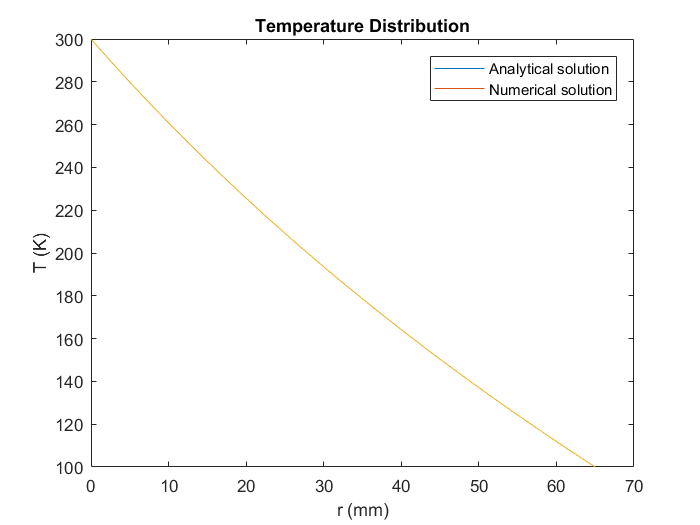
\includegraphics[width=0.8\linewidth]{Figures/tempereture_distribution_disk.png}
	\caption{Analytical and numerical temperature distribution}
    \label{antemp}
\end{figure}

\begin{figure} [H]
	\centering
	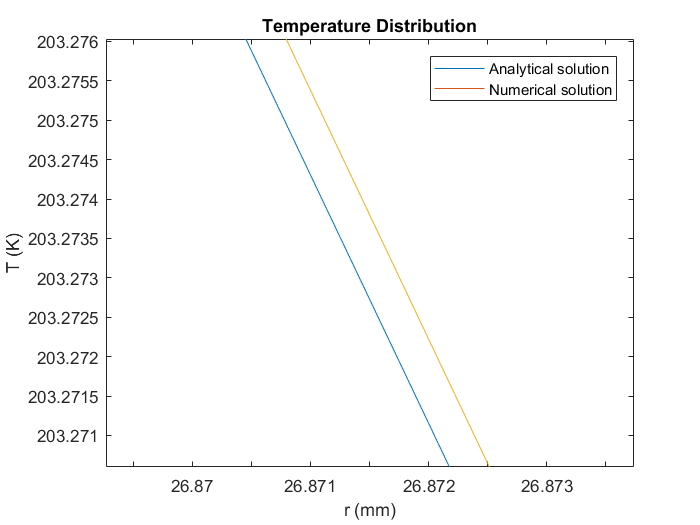
\includegraphics[width=0.8\linewidth]{Figures/tempereture_distribution_disk_zoom.png}
	\caption{Analytical and numerical temperature distribution close-up}
    \label{antempclose}
\end{figure}

\begin{figure} [H]
	\centering
	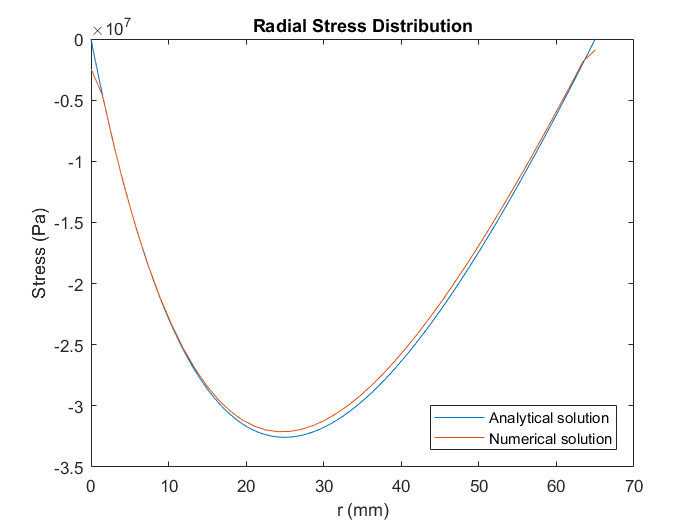
\includegraphics[width=0.8\linewidth]{Figures/Radialstressfulldisk.png}
	\caption{Analytical and numerical radial stress distribution}
    \label{numanaradstress}
\end{figure}

\begin{figure} [H]
	\centering
	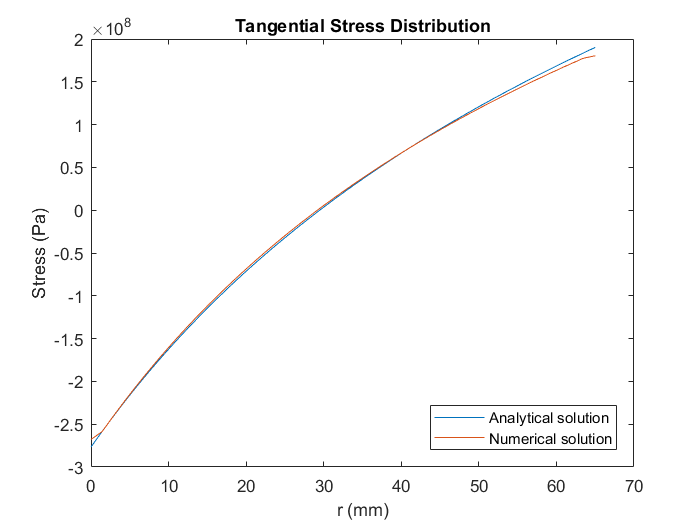
\includegraphics[width=0.8\linewidth]{Figures/Tangentialstressfulldisk.png}
	\caption{Analytical and numerical tangential stress distribution}
    \label{numanatanstress}
\end{figure}



\subsection{c}

The finite element model of the 1/22 part of the disk was created. It will be compared against the results of the full disk and the analytical solution. The temperature comparison has been left out since, it is again too similar to see any differences. The radial stress comparison can be seen in figure \ref{radtotal} and the tangential stress comparison in \ref{tantotal}.

From these comparisons a couple things become clear. The radial stress of the 1/22 part gets much closer to zero at the edges than the whole disk, an explanation for this could be the fact that the 1/22 part had a smaller mesh size. The tangential stress is also a bit closer to the analytical result for the 1/22 part than the whole disk, this difference can again be attributed to the smaller mesh size. 

\begin{figure} [H]
	\centering
	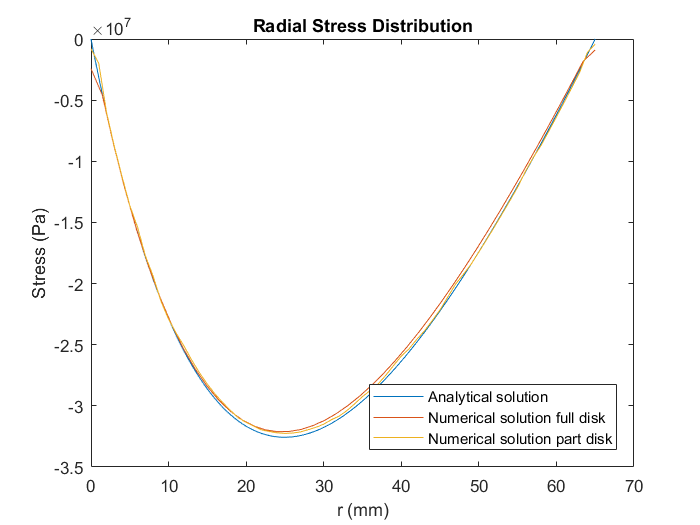
\includegraphics[width=1\linewidth]{Figures/Radialstresstotal.png}
	\caption{Radial stress distribution}
    \label{radtotal}
\end{figure}

\begin{figure} [H]
	\centering
	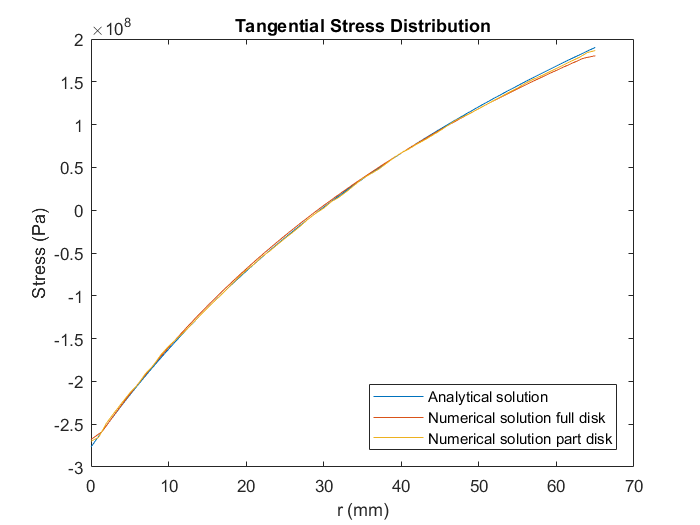
\includegraphics[width=1\linewidth]{Figures/tangentialstresstotal.png}
	\caption{Tangential stress distribution}
    \label{tantotal}
\end{figure}

\newpage